\chapter{一维Logistic映射的状态网络分析}

\section{定点域上一维混沌映射的基本性质}

给定映射$f$: $[0, 1]\rightarrow [0, 1]$,定点运算精度$n$和量化策略,可通过以下方式构造对应的状态映射网络$F_n$:
$1)$将$2^n$个可能状态看作$2^n$个节点;$2)$若$f(i/2^n)=j/2^n$,则节点$i$指向节点$j$。
为了表述方便,我们下面用$f_n(i)$来表示$f(i/2^n)$。令
\begin{equation*}
F_n(i)=\mathrm{R}\left(f_n(i)\cdot 2^n\right),
\end{equation*}
其中$\mathrm{R}(\cdot)$为量化函数,例如向下取整、向上取整和四舍五入
(这里只考虑四舍五入)。

根据上述定义,可以很容易证明以下关于$F_n$和$F_{n+1}$之间关系的性质。
\begin{Property}
\label{prop:evenrelation}
$F_{n+1}$中节点$(2i)$和$F_{n}$中节点$i$满足关系
\begin{equation}
F_{n+1}(2i)-2F_n(i)=
\begin{cases}
1          &  r_n\in [0.25, 0.5); \\
-1         &  r_n\in [0.5, 0.75); \\
0          &  \text{其他},
\end{cases}
\label{even_condition2}
\end{equation}
其中
\begin{equation*}
r_n=\mathrm{frac}(f_{n}(i)\cdot 2^n),
\end{equation*}
$\mathrm{frac}(x)=x-\lfloor x\rfloor$, $i\in \{0, \cdots, 2^n\}$,
$\lfloor x\rfloor$ 表示不大于实数$x$的最大整数。
\end{Property}
\begin{proof}
因为$F_{n+1}(2i)=\mathrm{R}\left(2\cdot f_{n+1}(2i)\cdot 2^{n}\right)$,另外,
\begin{equation}
f_{n+1}(2i)\equiv f_n(i),
\end{equation}
根据上述条件可推知
\begin{equation*}
F_{n+1}(2i)-2F_n(i)=\mathrm{R}\left(2\cdot f_{n}(i)\cdot 2^{n}\right)-\mathrm{R}\left(f_{n}(i)\cdot 2^{n}\right).
\end{equation*}

又因为
\begin{equation*}
\mathrm{R}(2 x)=2\cdot \mathrm{R}(x)+
\begin{cases}
0   &  0    \le \mathrm{frac}(x)<0.25;\\
1   &  0.25 \le \mathrm{frac}(x)<0.5; \\
-1  &  0.5  \le \mathrm{frac}(x)<0.75;\\
0   &  0.75 \le \mathrm{frac}(x)\le 1,
\end{cases}
\label{con:error}
\end{equation*}
从而上述性质得以直接证明。\qedsymbol
\end{proof}

\begin{Property}
\label{property:odd}
$F_{n+1}$中节点$(2i+1)$和$F_{n}$中节点$i$满足关系
\begin{eqnarray}
\left|F_{n+1}(2i+1)-2\cdot F_{n}(i)\right|
& \le &    \left|\mathrm{R}\left( (f_{n+1}(2i+1)
                            -f_{n+1}(2i))\cdot 2^{n+1} \right) \right|\nonumber\\
&     &    \hspace{1cm}   \label{eq:oddCondition}
\quad+\begin{cases}
2  & r_n\in [0.25, 0.75);\\
1  & \text{其他},
\end{cases}
\end{eqnarray}
其中$i\in \{0, \cdots, 2^n-1\}$。
\end{Property}
\begin{proof}
根据绝对值三角不等式$|a+b|\le |a|+|b|$可得
\begin{eqnarray}
\left|F_{n+1}(2i\!+\!1)\!-\!2\cdot F_n(i)\right|
& \le &   \left|F_{n+1}(2i\!+\!1)\!-\!F_{n+1}(2i)\right|\!+\!|F_{n+1}(2i)\!-\!2\cdot F_n(i)|.
\label{eq:TriangleInequ}
\end{eqnarray}

对任意实数$x$,$y$,恒有
\begin{equation}
\label{eq:integer}
|\mathrm{R}(x)-\mathrm{R}(y)|\leq |\mathrm{R}(x-y)|+1.
\end{equation}
因此
\begin{eqnarray}
\left|F_{n+1}(2i\!+\!1)\!-\!F_{n+1}(2i)\right|
& =   &  \left| \mathrm{R}\left(f_{n+1}(2i\!+\!1)\cdot 2^{n+1}\right)
                \!-\!\mathrm{R}\left(f_{n+1}(2i)\cdot 2^{n+1}\right) \right| \nonumber \\
& \le &  \left| \mathrm{R}\left(f_{n+1}(2i\!+\!1)\cdot 2^{n+1}
                \!-\!f_{n+1}(2i)\cdot 2^{n+1}\right) \right| \!+\!1.  \label{uppound}
\end{eqnarray}
将上述不等式和等式~(\ref{even_condition2})代入不等式~(\ref{eq:TriangleInequ}),该性质即可得证。\qedsymbol
\end{proof}

\begin{Property}
\label{property:odd2}
$F_{n+1}$中节点$(2i-1)$和$F_{n}$中节点$i$满足关系
\begin{eqnarray}
\left|F_{n+1}(2i-1)-2\cdot F_{n}(i)\right|
& \le &    \left|\mathrm{R}\left( (f_{n+1}(2i-1)
                    -f_{n+1}(2i))\cdot 2^{n+1} \right)\right|\nonumber\\
&     &    \hspace{1cm}
\quad+\begin{cases}
2  & r_n\in [0.25, 0.75);\\
1  & \text{其他},
\end{cases}
\end{eqnarray}
其中$i\in \{1, \cdots, 2^n\}$。
\end{Property}
\begin{proof}
根据绝对值三角不等式$|a+b|\le |a|+|b|$可得
\begin{eqnarray}
\left|F_{n+1}(2i\!-\!1)\!-\!2\cdot F_n(i)\right|
& \le &   \left|F_{n+1}(2i\!-\!1)\!-\!F_{n+1}(2i)\right|\!+\!|F_{n+1}(2i)\!-\!2\cdot F_n(i)|.
\label{eq:TriangleInequ2}
\end{eqnarray}
根据性质~\ref{property:odd2},应用不等式~(\ref{eq:integer})可得
\begin{eqnarray}
\left|F_{n+1}(2i\!-\!1)\!-\!F_{n+1}(2i)\right|
& =   &  \left| \mathrm{R}\left(f_{n+1}(2i\!-\!1)\cdot 2^{n+1}\right)
                \!-\!\mathrm{R}\left(f_{n+1}(2i)\cdot 2^{n+1}\right) \right| \nonumber \\
& \le &  \left| \mathrm{R}\left(f_{n+1}(2i\!-\!1)\cdot 2^{n+1}
                \!-\!f_{n+1}(2i)\cdot 2^{n+1}\right) \right| \!+\!1.  \label{uppound}
\end{eqnarray}
将上述不等式和等式~(\ref{even_condition2})代入不等式~(\ref{eq:TriangleInequ2})中,该性质即可得证。\qedsymbol
\end{proof}

\section{定点域上Logistic映射的性质分析}

\subsection{数字化Logistic映射的定义}

Logistic映射是研究动力系统、混沌、分形等复杂系统行为的一个经典模型,早在20世纪50年代,就被生态学家用来描述种群的变化,
在保密通信领域的应用也十分广泛,其数学表达式为
\begin{equation}
f(x)=\mu\cdot x\cdot (1-x),
\label{eq:logistic}
\end{equation}
其中$x\in [0,1]$,$\mu\in (0,4]$。

在精度为$n$的定点运算域上,Logistic映射$f(x)=\mu\cdot x\cdot (1-x)$变为
\begin{equation}
f_n(i)=(N_{\mu}/2^{n_\mu})\cdot (i/2^n) \cdot (1-i/2^n),
\label{eq:LogisticFinite}
\end{equation}
其中$N_{\mu}$属于集合$\{0, \cdots, 2^{n_\mu+2}\}$里的奇数,$\mu=N_{\mu}/2^{n_\mu}$,且$n_\mu \le n$。

图~\ref{fig:networkLogistic5and6bits}为相同控制参数、不同运算精度下Logistic映射的状态映射网络。

\begin{figure}[!htb]
\centering
\begin{minipage}{0.8\ThreeImW}
\centering
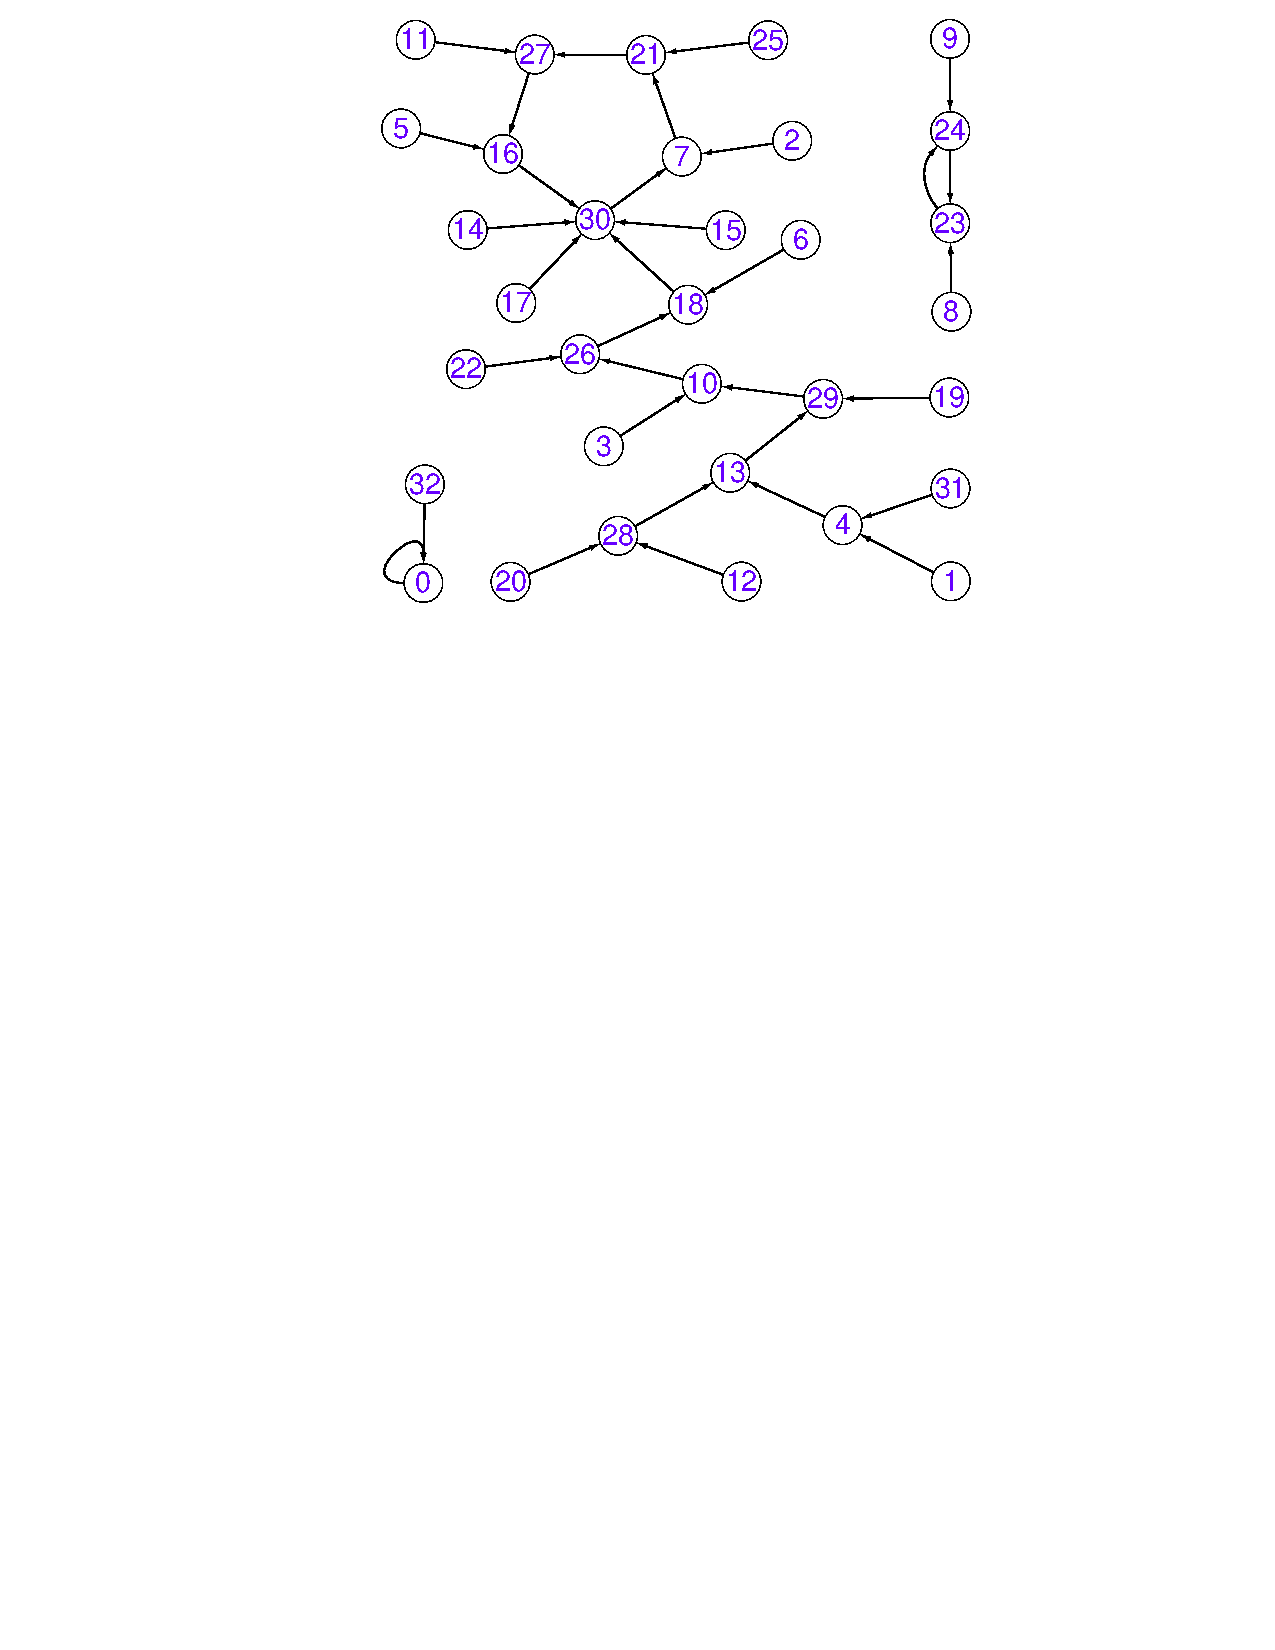
\includegraphics[width=0.8\ThreeImW]{n5round_u121}
a)
\end{minipage}\hspace{0.3\figsep}
\begin{minipage}{\ThreeImW}
\centering
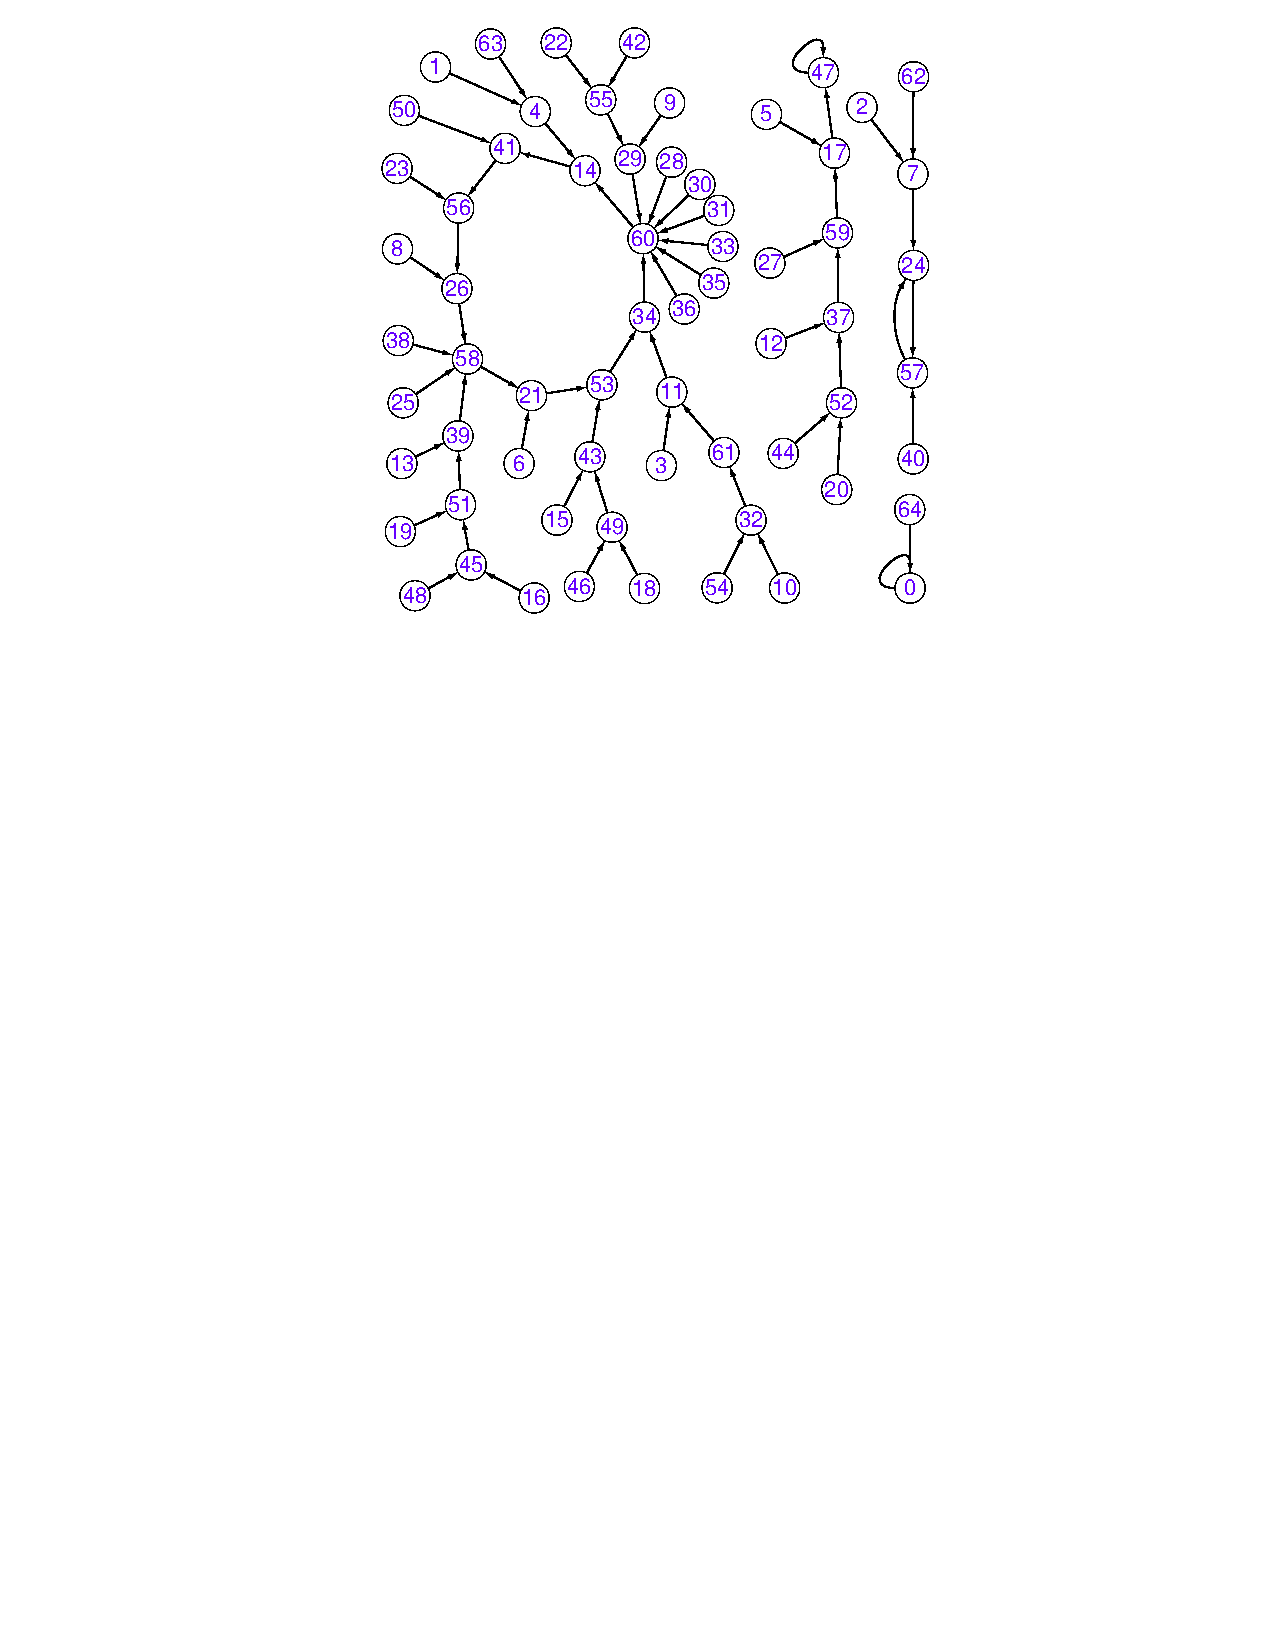
\includegraphics[width=\ThreeImW]{n6round_u242}
b)
\end{minipage}\hspace{0.3\figsep}
\begin{minipage}{1.2\ThreeImW}
\centering
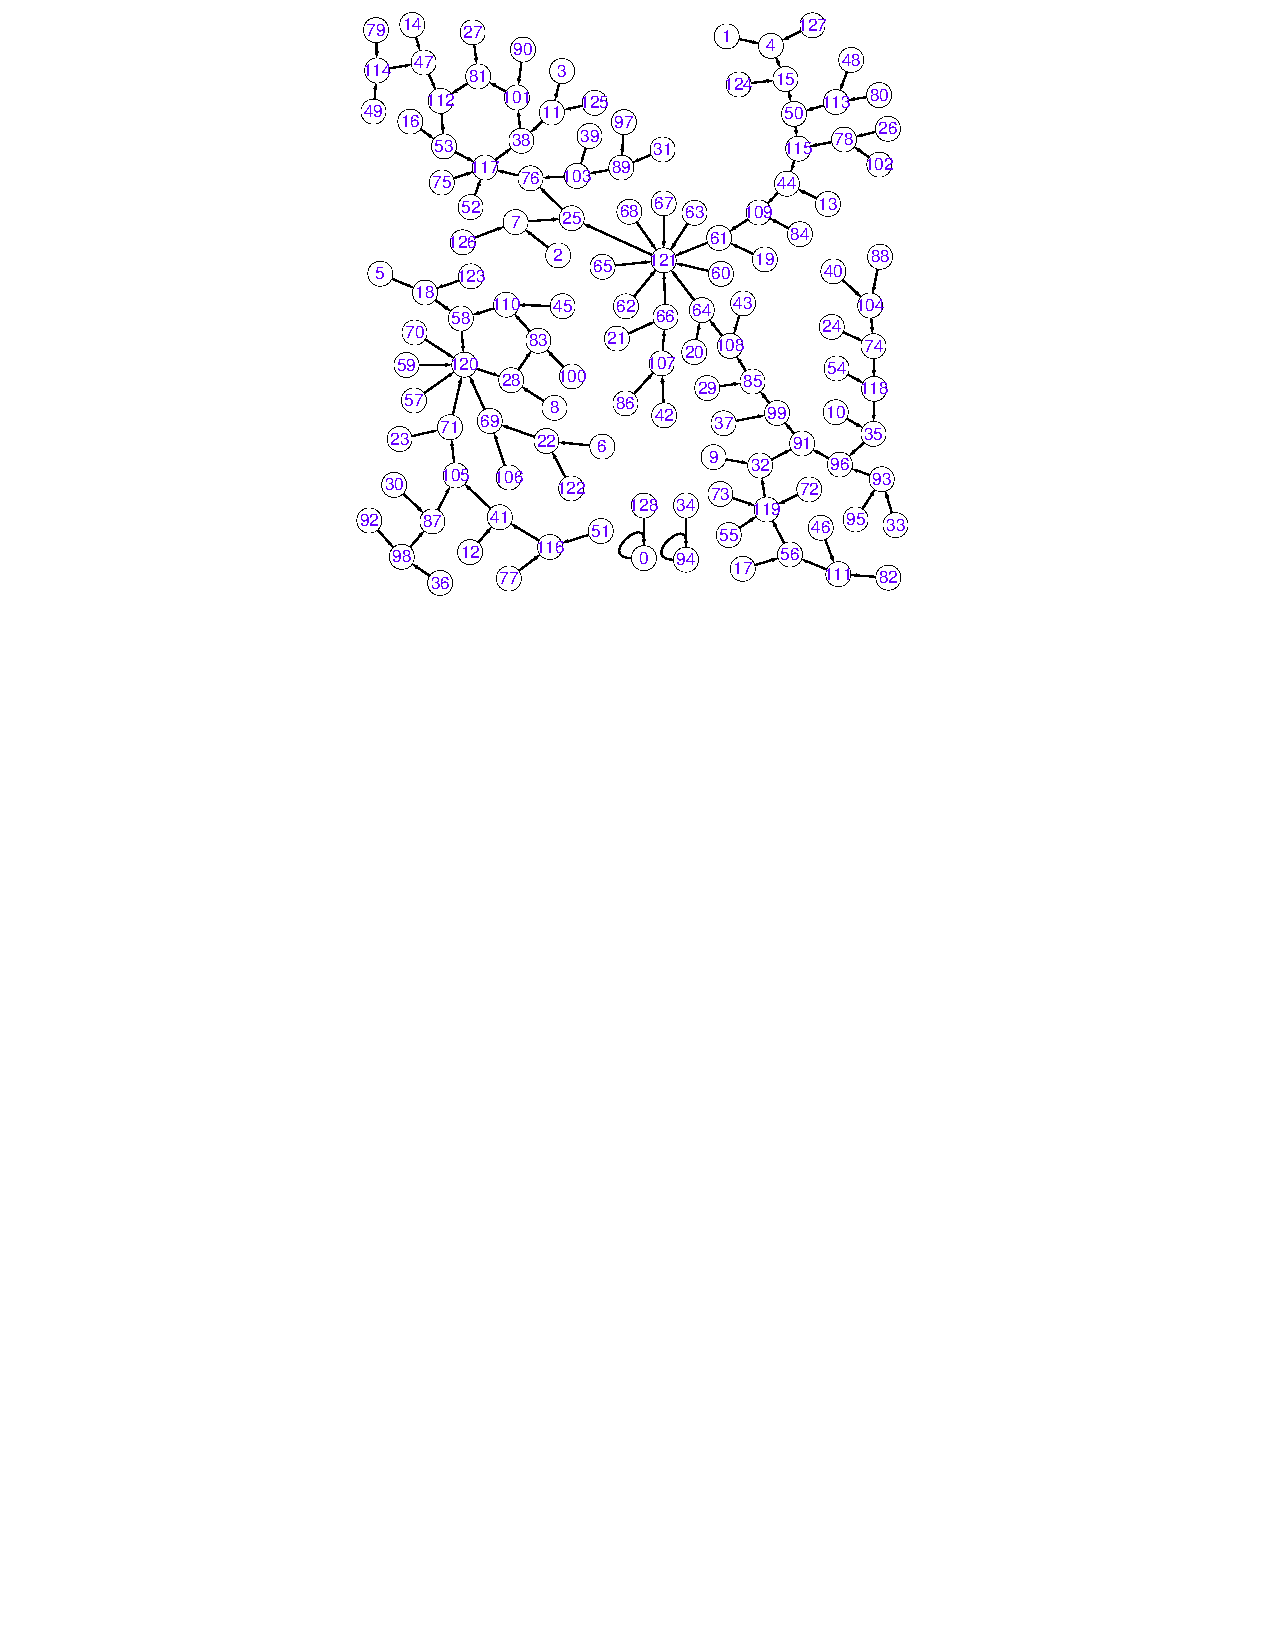
\includegraphics[width=1.2\ThreeImW]{n7round_u484}
c)
\end{minipage}
\caption{控制参数$\mu=121/2^5$时,Logistic映射的状态映射网络:
a) 5比特精度; b) 6比特精度; c) 7比特精度}
\label{fig:networkLogistic5and6bits}
\end{figure}

\iffalse
通过上述不同定点运算精度下Logistic映射的状态映射网络,可以初步观察到数字混沌系统的状态映射网络具有以下基本特征:\fi
从图~\ref{fig:networkLogistic5and6bits}可观察到数字混沌系统状态映射网络的如下基本特征:
\begin{itemize}
\item 整个状态映射网络由少量弱连通分量构成。(弱连通分量是有向图的最大子图;有向图中任意两点之间有且只有一条有向路径相连。)

\item 每个弱连通分量有且仅有一个自环或环路。

\item 弱连通分量中的每个节点经过一个“暂态”过程都会连向其循环。
\end{itemize}

从图~\ref{fig:networkLogistic5and6bits}可以进一步观察到,Logistic映射的状态映射网络具有以下特征,
即最大弱连通分量的节点数占整个状态映射网络节点数的一半以上\upcite{wang2004periodicity}。

\subsection{Logistic映射的状态映射网络与实现精度之间的关系}

\begin{Corollary}
\label{coro:logisticoddUpper}
$F^*_{n+1}$中节点$(2i+1)$和$F^*_{n}$中节点$i$满足关系
\begin{equation*}
\left|F^*_{n+1}(2i+1)-2\cdot F^*_n(i)\right|\le
\begin{cases}
6  & r_n \in [0.25, 0.75);\nonumber\\
5  & \mbox{其他},
\end{cases}
\end{equation*}
其中$i\in \{0, \cdots, 2^n-1\}$,且$n\ge 3$。
\end{Corollary}

\begin{proof}
将等式~(\ref{eq:LogisticFinite})带入不等式~(\ref{eq:oddCondition}),可得
\begin{eqnarray*}
\left|F^*_{n+1}(2i+1)-2\cdot F^*_n(i)\right|
& \le & \left|\mathrm{R}\left( \left(N_{\mu}/2^{n_\mu+2}\right)
                 \cdot \left(4-(1+4i)/2^{n-1}\right)\right)\right| \\
&     & \hspace{1cm}
\quad+\begin{cases}
2  & r_n \in [0.25, 0.75); \\
1  & \mbox{其他}.
\end{cases}
\end{eqnarray*}

由于$(N_{\mu}/2^{n_\mu+2})\in [0, 1]$,进一步可得
\begin{eqnarray}
\left|F^*_{n+1}(2i+1)-2\cdot F^*_n(i)\right|
& \le & \left|\mathrm{R}\left(4-(1+4i)/2^{n-1}\right)\right|+
\begin{cases}
2  & r_n \in [0.25, 0.75);\nonumber\\
1  & \mbox{其他},
\end{cases}\\
& \le &
\begin{cases}
6  & r_n \in [0.25, 0.75);\nonumber\\
5  & \mbox{其他}.
\end{cases}
\end{eqnarray}\qedsymbol
\end{proof}

\begin{figure}[!htb]
\centering
\begin{minipage}{\TwoImW}
\centering
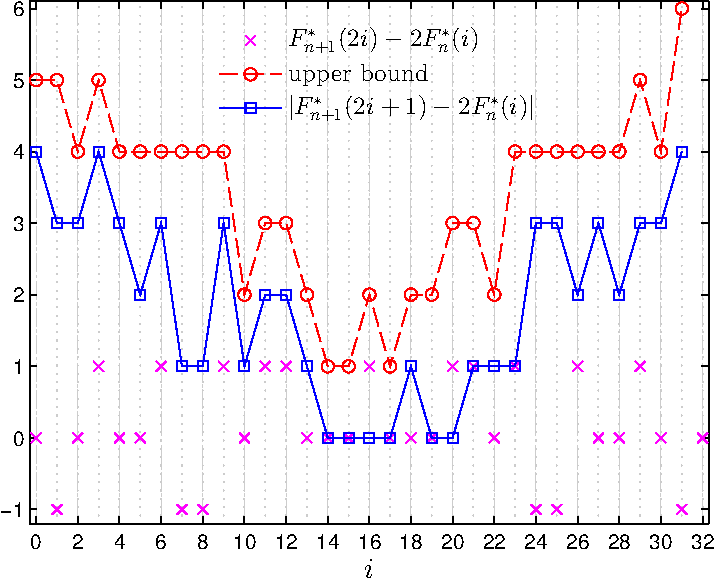
\includegraphics[width=\TwoImW]{upper_bound_add}
a)
\hspace{1mm}
\end{minipage}
\begin{minipage}{\TwoImW}
\centering
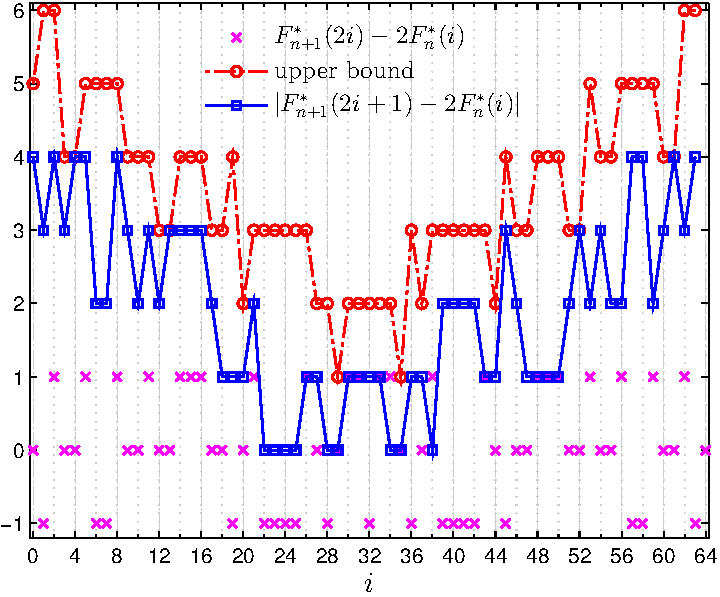
\includegraphics[width=\TwoImW]{upper_bound_add2}
b)
\end{minipage}
\caption{$F^*_n$与$F^*_{n+1}$中对应节点的差值分布: a) $n=5$; b) $n=6$}
\label{fig:upperbound}
\end{figure}

根据推论~\ref{coro:logisticoddUpper}可知,$|F^*_{n+1}(2i+1)-2\cdot F^*_n(i)|$的上界取决于$i$和$N_{\mu}$。
图~\ref{fig:upperbound} a)为图~\ref{fig:networkLogistic5and6bits} a)中每个节点对应的差值
$|F^*_{n+1}(2i+1)-2\cdot F^*_n(i)|$和$F^*_{n+1}(2i)-2F^*_n(i)$,为进一步分析比较$F^*_{n}$和$F^*_{n+1}$的关系,
图~\ref{fig:networkLogistic5and6bits} b)中每个节点对应的差值如图~\ref{fig:upperbound} b)所示。

\begin{Property}
状态映射网络$F^*_{n_\mu}$对$F^*_{n}$有决定性影响。
\label{prop:dominate}
\end{Property}
\begin{proof}
根据性质~\ref{prop:evenrelation}和推论~\ref{coro:logisticoddUpper},$F^*_{n}$可由$F^*_{j}$逐步演化而来,
其中$j=n_\mu\sim n$。因为演化前后状态映射网络对应节点的量化误差可控,因此$F^*_{n_\mu}$的初始结构对$F^*_{n}$
有决定性影响。\qedsymbol
\end{proof}

\subsection{Logistic映射SMN入度分布的理论推导}

\begin{theorem}
Logistic映射对应状态映射网络$F^*_n$的节点累积入度分布满足关系
\begin{equation*}
P(k)=\left(\frac{2}{\mu k}-\frac{k}{2^{n+1}}\right)^2.
\end{equation*}
\label{theorem:logisticMap}
\end{theorem}
\begin{proof}
给定量化策略,在精度为$n$的定点运算域上,任意一维映射的定义域和值域可被等间隔划分,其中$\Delta=1/2^n$,如图~\ref{fig:degree}所示。

\begin{figure}[!htb]
\centering
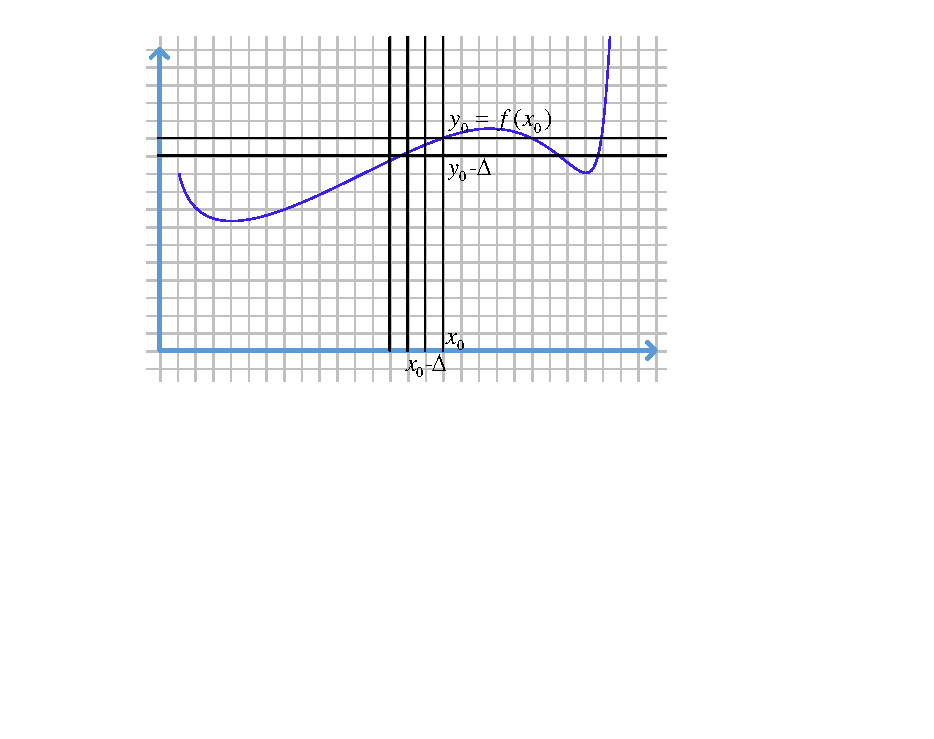
\includegraphics[width=1.25\BigOneImW]{degree}
\caption{数字域上映射原像对应的区间数}
\label{fig:degree}
\end{figure}

对$y_0=f(x_0)$所在区间,其原像对应区间的个数为
\begin{equation*}
c=\left\lceil \frac{ |x-f^{-1}(f(x)-\Delta)| }{\Delta} \right\rceil,
\end{equation*}
其中$\lceil x \rceil$表示大于等于实数$x$的最小整数。
由于Logistic映射~(\ref{eq:logistic})具有对称性,即
\begin{equation}
f(x)=f(1-x),
\label{eq:logisticsym}
\end{equation}
所以对应$y=f(x)$的节点入度等于定义域左半部分入度的两倍。

映射~(\ref{eq:logistic})的反函数为
\begin{equation*}
f^{-1}(y)=\left(1-\sqrt{1-4y/\mu}\right)/2,\ x\in [0, 1/2).
\end{equation*}
当$x\in [0, 1/2)$时,$f'(x)=\mu \cdot (1-2x)>0$,$f(x)$关于$x$单调递增。因此对应$y=f(x)$的节点入度为
\begin{eqnarray*}
k & = &  2 \cdot \left\lceil \frac{ f^{-1}(y)-f^{-1}(y-1/2^n)}{2^{-n}} \right\rceil \\
  & = &  2 \cdot \left\lceil \frac{\sqrt{1-4(y-1/2^n)/ \mu} -\sqrt{1-4y/ \mu} }{2^{1-n}} \right\rceil.
\end{eqnarray*}
根据上式,可得
\begin{equation}
y=\frac{\mu}{4} -\frac{1}{\mu\cdot  (k-\epsilon)^2 }
-\frac{\mu\cdot (k-\epsilon)^2}{2^{2n+4}} + 2^{-n-1},
\label{eq:expressy}
\end{equation}
其中$\epsilon$为量化误差,且$0\le \epsilon<2$。

由于误差$\epsilon$在推导过程中产生的影响较小,因此在下面的讨论中忽略误差项。\\
状态$y$的秩为
\begin{equation*}
r=\left\lceil \frac{\mu/4-y}{1/2^{n}} \right\rceil,
\end{equation*}
状态映射网络节点数为
\begin{equation*}
N=\left\lceil \frac{\mu/4}{1/2^{n}}\right\rceil.
\end{equation*}
根据累积分布的定义,则有
\begin{equation*}
P(k)=1-\frac{4y}{\mu}.
\end{equation*}
将等式~(\ref{eq:expressy})代入上式,从而可得
\begin{equation*}
P(k)=\left( \frac{2}{\mu k}- \frac{k}{2^{n+1}} \right)^2.
\end{equation*}

根据上述推导可知,$P(k)$关于$n$单调增加,因此随着$n$的增大,Logistic映射的状态映射网络中节点的累积入度分布$P(k)$趋于其极限:
\begin{equation}
\lim\limits_{n \to \infty}P(k)=\frac{4}{\mu^{2}k^{2}}.
\end{equation}\qedsymbol
\end{proof}

\begin{figure}[!htb]
\centering
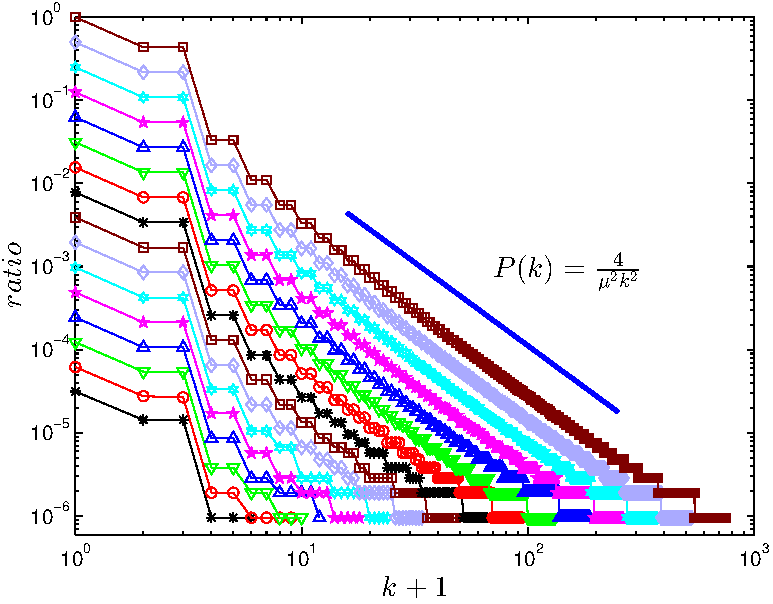
\includegraphics[width=1.25\BigOneImW]{CumulativeInDegreeDistribution_u121_n_5_20}
\caption{状态映射网络$F^*_{5} \sim F^*_{20}$的节点累积入度分布,其中$\mu=\frac{121}{2^{5}}$}
\label{fig:CumulativeInDegreeDistribution_u121_n_5_20}
\end{figure}

\begin{figure}[!htb]
\centering
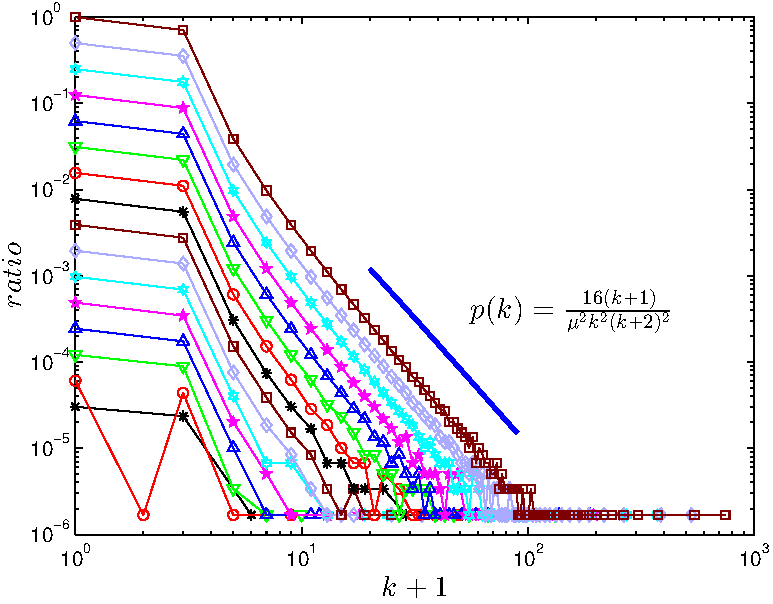
\includegraphics[width=1.25\BigOneImW]{InDegreeDistribution_u121_n_5_20}
\caption{状态映射网络$F^*_{5} \sim F^*_{20}$的节点入度分布,其中$\mu=\frac{121}{2^{5}}$}
\label{fig:InDegreeDistribution_u121_n_5_20}
\end{figure}

\begin{Corollary}
\label{coro:indegreedistribute}
Logistic映射对应状态映射网络$F^*_n$的节点入度分布满足关系
\begin{equation*}
p(k)\doteq \frac{16(k+1)}{\mu^{2}k^{2}(k+2)^{2}}.
\end{equation*}
\end{Corollary}
\begin{proof}
由于Logistic映射具有对称性,所以除驻点$f(1/2)$外,其状态映射网络的节点入度均为偶数。

根据累积入度分布的定义,入度分布$p(k)$可表示为
\begin{equation*}
p(k)=P(k)-P(k+2).
\end{equation*}
从而可得
\begin{eqnarray*}
p(k) & = & \left( \frac{2}{\mu k}- \frac{k}{2^{n+1}} \right)^2 - \left( \frac{2}{\mu (k+2)}
                 - \frac{k+2}{2^{n+1}} \right)^2\\
     & = & (k+1) \left(\frac{16}{\mu^2 k^2 (k+2)^2} - \frac{1}{2^{2n}} \right).
\end{eqnarray*}
根据上述结论可知,随着$n$的增大,Logistic映射的状态映射网络中节点的入度分布$p(k)$逐渐趋于其极限:
\begin{equation}
\lim\limits_{n \to \infty} p(k)=\frac{16(k+1)}{\mu^2 k^2 (k+2)^2}.
\end{equation}\qedsymbol
\end{proof}

图~\ref{fig:CumulativeInDegreeDistribution_u121_n_5_20}、图~\ref{fig:InDegreeDistribution_u121_n_5_20}分别为
Logistic映射的状态映射网络中节点的累积入度分布和入度分布,这里$N_{min}=2^{5}$,$N_{max}=2^{20}$。

\section{浮点域上Logistic映射的性质分析}

考虑到科学研究和工程技术中数的表示范围和表示精度,现代数字计算机采用两种二进制表示形式来表示实数,即定点格式和浮点格式。
前者适用于表示具有固定精度的整数或实数,而后者适用于近似表示具有较高精度的实数,但浮点数的表示范围越大, 浮点数的表示精度就降低。
在浮点数标准被确定之前,不同的数字计算机采用不同的二进制表示形式来进行浮点运算。
之后浮点数通常以IEEE 754标准存储在数字计算机中,其在内存中的表示形式如下图~\ref{fig:IEEE_float}所示,
其中$s$表示浮点数的符号,$exponent$反映浮点数的表示范围,$mantissa$反映浮点数的精度。
\begin{figure}[!htb]
\centering
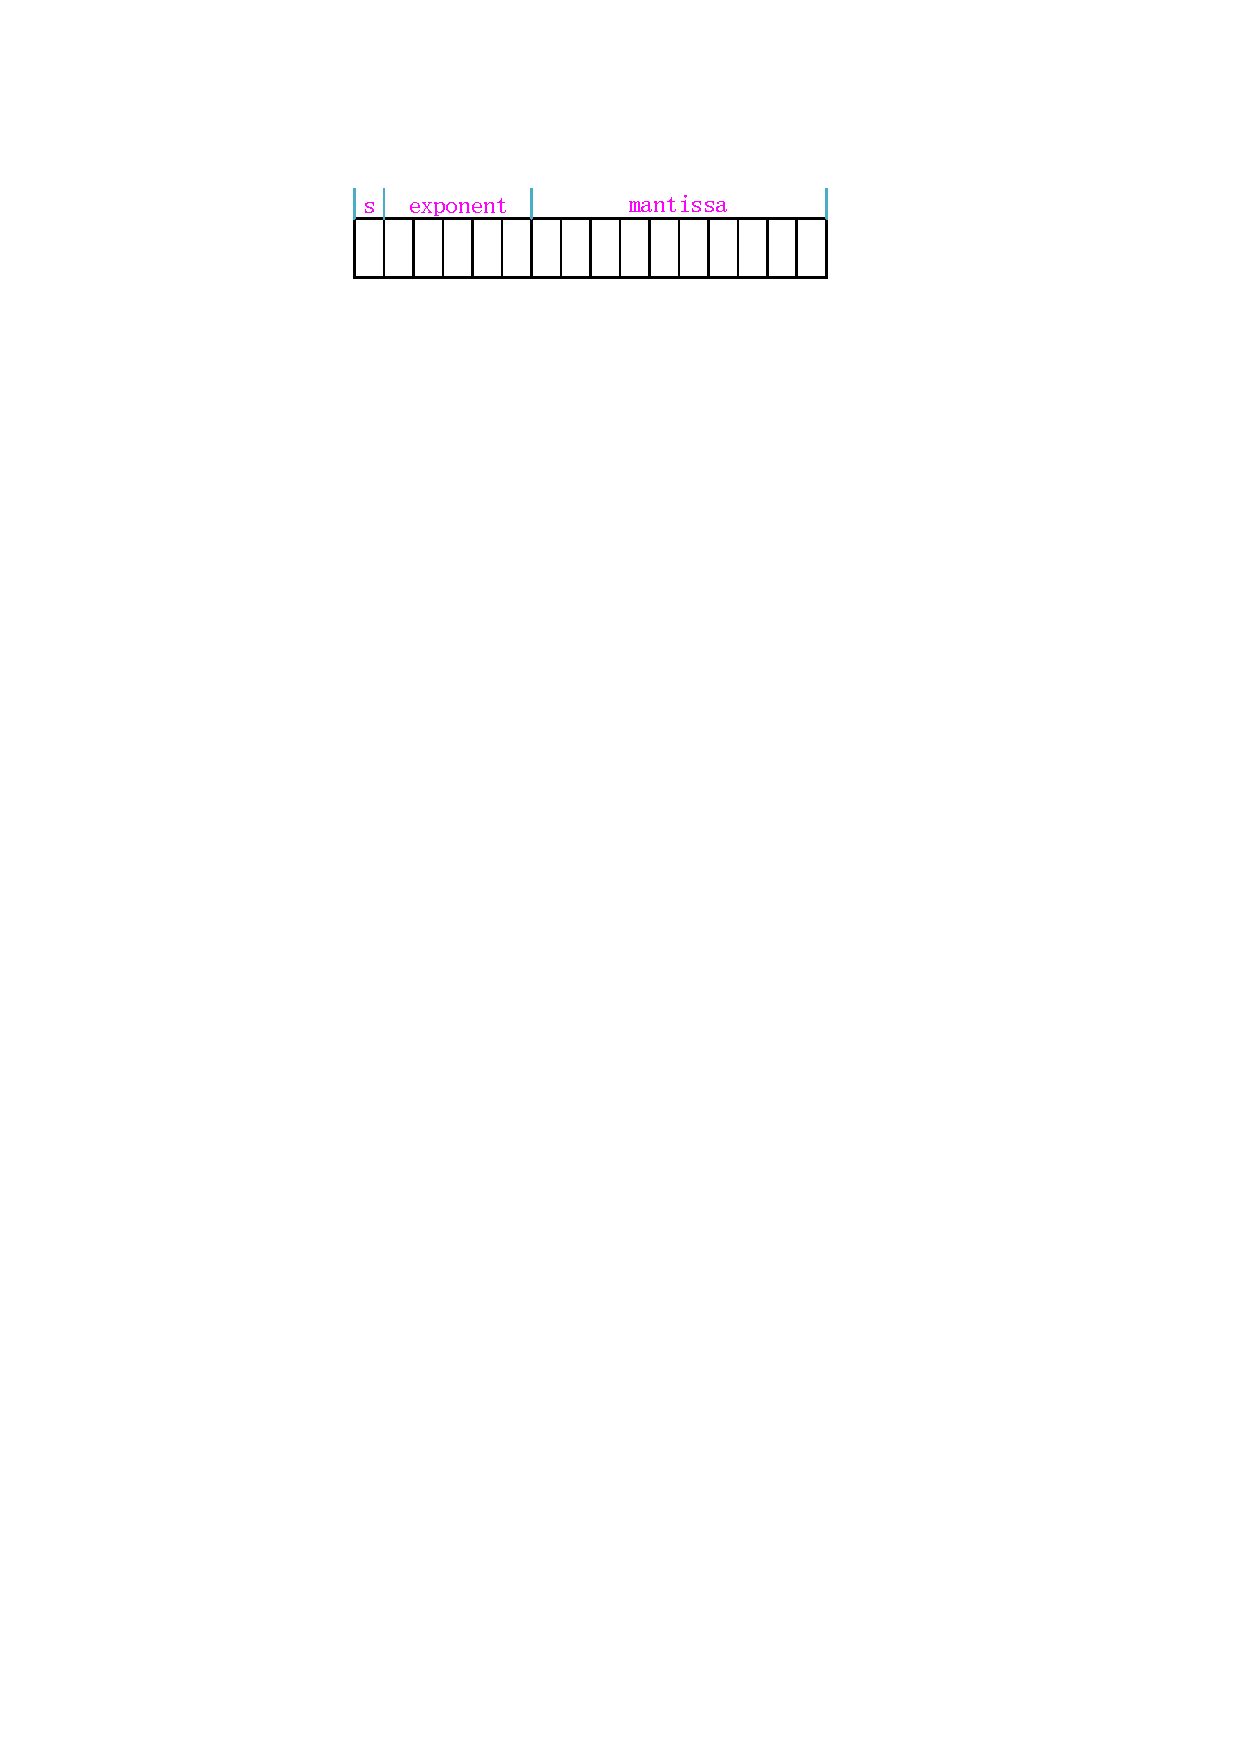
\includegraphics[width=1.25\BigOneImW]{float_point_format1}
\caption{浮点数在计算机内存中的表示形式}
\label{fig:IEEE_float}
\end{figure}

浮点数$\{b_i\}_{i=0}^{n-1}$的值为尾数与2的指数幂的乘积:
\begin{eqnarray*}
v=
\begin{cases}
  0                                                                              & e=0, \mathit{os}=0;        \\
  (-1)^{s}\cdot \left(\sum\limits_{i=1}^m b_{l+i}   \cdot 2^{-i}\right)\cdot 2^{2-2^{l-1}}  & e=0, \mathit{os}\neq 0;    \\
  (-1)^{s}\cdot \infty                                                           & e=2^l-1, \mathit{os}=0;    \\
  \mbox{NaN}                                                         & e=2^l-1, \mathit{os}\neq 0; \\
  (-1)^{s}\cdot \left(1+\sum\limits_{i=1}^{m} b_{l+i} \cdot 2^{-i} \right)\cdot 2^{e-\mathit{os}}
                                                                                 & \text{其他},
\end{cases}
\end{eqnarray*}
其中$s=b_0$,$e=\sum\limits_{i=0}^{l-1} b_{1+i} \cdot 2^{i}$,$\mathit{os}=2^{l-1}-1$。

对于单精度浮点数(binary32),$(l, m)=(8, 23)$,例如C语言中的``float"类型和Matlab中的``single"类型;
对于双精度浮点数(binary64),$(l, m)=(11, 52)$,例如C语言中的``double"类型和Matlab中的``double"类型;
对于IEEE 754-2008标准中的半精度浮点数(binary16),$(l, m)=(5, 10)$,其适用于对精度要求较低,对存储空间
要求较高的场合。由于半精度浮点数(binary16)的表示范围相对较小,故其被广泛用于科学研究和数值仿真\upcite{Rau:binary16}。

在浮点运算域上,由于量化误差的存在,等式~(\ref{eq:logisticsym})通常不成立,例如在binary16环境下,
$x=0.0099945068359375$时,$f(x)\neq f(1-x)$,如表~\ref{tab:differenceLogistic}所示。

\begin{table*}[!htb]
\centering
\caption{Binary16环境下$f(x)\neq f(1-x)$的部分情况}
\resizebox{\textwidth}{28mm}{
\begin{tabular}{c *{4}{|c}}
\hline
$x$    &  $1-x$ & $1-(1-x)$  &   $f(x)$  &   $f(1-x)$ \\ \hline
0.0099945068359375 & 0.98974609375 & 0.01025390625 & 0.037384033203125 & 0.038360595703125\\ \hline
0.04998779296875 & 0.94970703125 & 0.05029296875 & 0.179443359375 & 0.1805419921875\\ \hline
0.0899658203125  & 0.90966796875 & 0.09033203125 & 0.309326171875 & 0.310546875\\ \hline
0.0999755859375  & 0.89990234375 & 0.10009765625 & 0.340087890625 & 0.340576171875\\ \hline
0.199951171875   & 0.7998046875 & 0.2001953125 & 0.6044921875 & 0.60498046875\\ \hline
0.289794921875   & 0.7099609375 & 0.2900390625 & 0.77783203125 & 0.7783203125\\ \hline
0.389892578125   & 0.60986328125 & 0.39013671875 & 0.89892578125 & 0.8994140625\\ \hline
0.489990234375   & 0.509765625 & 0.490234375 & 0.9443359375 & 0.94482421875\\ \hline
\end{tabular}}
\label{tab:differenceLogistic}
\end{table*}

因为$\mathit{fl}(x)$与$\mathit{fl}(1- \mathit{fl}(1-\mathit{fl}(x)))$之间存在量化误差,所以
\begin{equation*}
\mu\cdot x\cdot (1-x)\stackrel{?}{=}\mu \cdot(1-x)\cdot \left(1-(1-x)\right)
\end{equation*}
不一定成立,$\mathit{fl}(x)$表示给定浮点运算域上最接近$x$的标准化浮点数。
如果一个数落在区间$[0.5, 1]$上,则$1-\mathit{fl}(x) = \mathit{fl}(1-\mathit{fl}(x))$,因此
\begin{equation}
\mathit{fl}(1- \mathit{fl}(1-\mathit{fl}(x)))\equiv
\begin{cases}
1- \mathit{fl}(1-\mathit{fl}(x))   &   x\leq 0.5; \\
\mathit{fl}(x)                     &   x>0.5.
\end{cases}
\label{Condition:flxtwo}
\end{equation}

对任意$x \in \mathbb{R}\cap [0, 1]$,存在唯一整数$e$使得$x=(\sum_{i=0}^\infty x_i\cdot 2^{-i})\cdot 2^e$,其中$x_0=1$。
浮点数$x$在计算机内存中的表示形式为
\begin{equation}
\mathit{fl}(x)=
\begin{cases}
(\sum_{i=1}^{m} x_i\cdot 2^{-i})\cdot 2^{2-2^{l-1}}  &  x\in (0,2^{2-2^{l-1}}); \\
(1+\sum_{i=1}^{m} x_i\cdot 2^{-i})\cdot 2^e          &  x\in [2^e,2^{e+1}),
\end{cases}
\end{equation}
其中$e\in \{2-2^{l-1}, \cdots, -2\}$,$l$表示阶码位数,$m$表示尾数位数。
根据上述表示,进而可得
\begin{eqnarray}
1-\mathit{fl}(x)=
\begin{cases}
\sum_{i=1}^{2^{l-1}-2} 2^{-i}+(\sum_{i=1}^{m} \bar{x}_i\cdot 2^{-i}+ 2^{-m})\cdot 2^{2-2^{l-1}} &  x\in (0,2^{2-2^{l-1}}); \\
\sum_{i=1}^{-(e+1)}2^{-i}+(\sum_{i=1}^{m} \bar{x}_i\cdot 2^{-i}+ 2^{-m} )\cdot 2^{e}            &  x\in [2^e,2^{e+1}),
\end{cases}
\label{1minusflx}
\end{eqnarray}
其中$\bar{x}_i=1-x_i$。由于等式~(\ref{1minusflx})第一种情况中$(1-\mathit{fl}(x))$的阶码为-1,故
\begin{equation}
\mathit{fl}( 1-\mathit{fl}(x))= \left(1+\sum_{i=1}^m \hat{x}_i\cdot 2^{-i} \right)\cdot 2^{-1},
\end{equation}
其中$\hat{x}_i\in\{0, 1\}$,$2^{l-1}-2\ge m+1$。
根据浮点数在计算机内存中的表示形式,等式~(\ref{1minusflx})可进一步表示为
\begin{eqnarray}
\mathit{fl}(1-\mathit{fl}(x))=
\begin{cases}
(\sum_{i=1}^{m+1} 2^{-i})                &   x\in (0,2^{2-2^{l-1}});   \\
(\sum_{i=1}^{m+1} 2^{-i})                &   x\in [2^{e_1},2^{e_1+1}); \\
(\sum_{i=1}^{-e_2-1} 2^{-i})+(\sum_{i=1}^{m+1+e_2} \bar{x}_i\cdot 2^{-i} )\cdot 2^{e_2}    &   x\in [2^{e_2},2^{e_2+1}),
\end{cases}
\label{fl1minusfx}
\end{eqnarray}
其中$e_1\in \{2-2^{l-1}, \cdots, -m-2\}$,$e_2\in \{-m-1, \cdots, -2\}$。

\begin{figure}[!htb]
\centering
\begin{minipage}{1.25\BigOneImW}
\centering
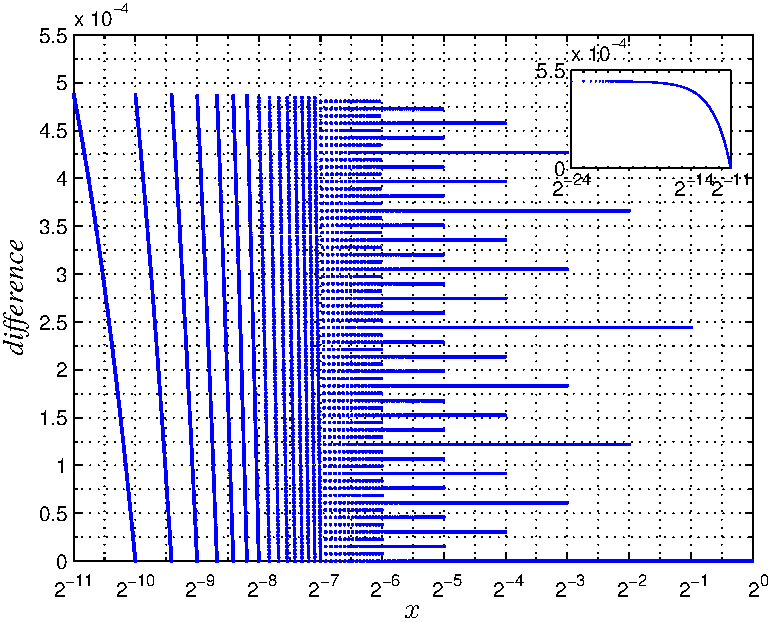
\includegraphics[width=1.25\BigOneImW]{x_diff}
\end{minipage}
\caption{Binary16中$1-(1-x)$与$x$的差值关于$x$的变化规律}
\label{fig:differencex}
\end{figure}

\begin{figure}[!htb]
\centering
\begin{minipage}{1.25\BigOneImW}
\centering
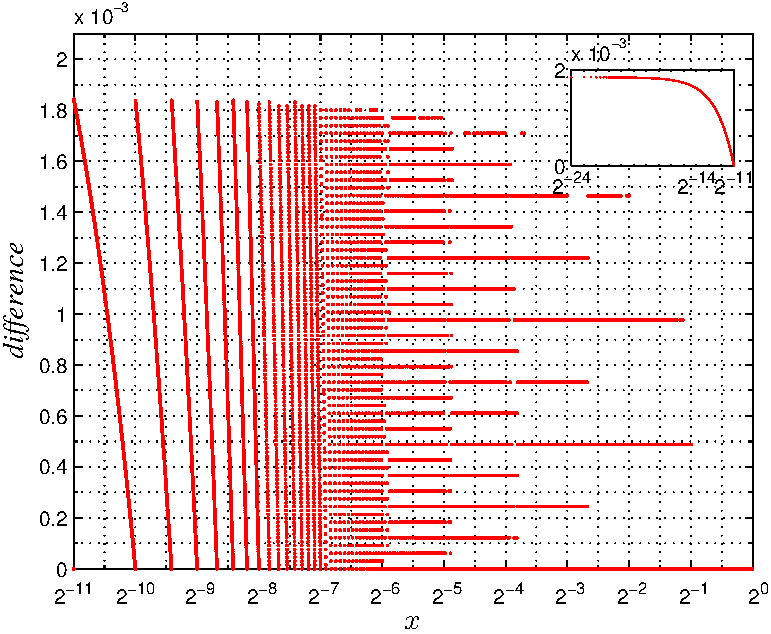
\includegraphics[width=1.25\BigOneImW]{fx_diff}
\end{minipage}
\caption{Binary16中$f(1-x)$与$f(x)$的差值关于$x$的变化规律}
\label{fig:differencefx}
\end{figure}

根据等式~(\ref{Condition:flxtwo})的第一种情况,等式~(\ref{1minusflx})与等式~(\ref{fl1minusfx})相减,则有
\begin{eqnarray}
\mathit{fl}(1&-&\mathit{fl}(1-\mathit{fl}(x)))-\mathit{fl}(x)
= (1-\mathit{fl}(x))-\mathit{fl}(1-\mathit{fl}(x)) \nonumber\\
&=&\begin{cases}
(\sum_{i=m+2}^{2^{l-1}-2} 2^{-i})
                          +(\sum_{i=1}^{m} \bar{x}_i\cdot 2^{-i}+ 2^{-m})\cdot 2^{2-2^{l-1}}   & x\in (0,2^{2-2^{l-1}}); \\
(\sum_{i=m+2}^{-(e_1+1)} 2^{-i})+(\sum_{i=1}^{m} \bar{x}_i\cdot 2^{-i}+ 2^{-m} )\cdot 2^{e_1}  & x\in [2^{e_1},2^{e_1+1}); \\
(\sum_{i=m+2+e_2}^{m} \bar{x}_i\cdot 2^{-i}+ 2^{-m} )\cdot 2^{e_2}                             & x\in [2^{e_2},2^{e_2+1}).
\end{cases}
\label{eq:xdiffer1_x}
\end{eqnarray}

根据等式~(\ref{eq:xdiffer1_x}),在数字计算机中,$1-(1-x)$与$x$的差值关于$x$分段单调递减,如图~\ref{fig:differencex}所示。
图~\ref{fig:differencex}右上角的插图对应等式~(\ref{eq:xdiffer1_x})的前两种情况,可以观察到,区间
$[2^{-10+2-2^4}, 2^{2-2^4}]=[2^{-24}, 2^{-14}]$和$\{[2^{e_1}, 2^{e_1+1}]\}_{e_1=2-2^4}^{-10-2}
=\{[2^{e_1}, 2^{e_1+1}]\}_{e_1=-14}^{-12}$的对应曲线可以平滑连接。类似的,$f(1-x)$与$f(x)$的差值关于$x$的变化规律
如图~\ref{fig:differencefx}所示。

\section{混沌伪随机数发生器的随机性检测}

伪随机数序列由数学表达式生成,但伪随机数并不是真正意义上随机,因为序列本身随着时间的推移必然会进入一个循环。对于伪随机数来说,衡量其序列随机性的指标主要有
均匀性、相关性和周期性。均匀性是指随机序列服从均匀分布;相关性是指伪随机数发生器生成的随机序列中各个随机数是否相关,随机数之间的相关性应尽可能弱;周期性是指经过多久,
随机序列进入循环,进入循环前的暂态分枝应尽可能长。由于混沌系统的不确定性、不可重复、不可预测等特性,混沌系统被广泛应用于设计伪随机数发生器,
因此各种基于混沌的伪随机数发生器应运而生
\upcite{Phatak:LogisticRNG:PRE95,kocarev2003pseudorandom,Addabbo:Tent:ITIM2006,heidari1994chaotic,Chen:random:CASII2010,
LiCY:PRNS:VLSI2012,HPhu:DCS:SMCS2015,addabbo2007class:TCASI,zhou1997precision}。
当我们在数字化应用中使用伪随机数发生器时,一个很重要的问题是如何检测混沌伪随机数发生器的随机性能。

SMN可对基于混沌的伪随机数发生器进行分类,并对其随机性进行检测\upcite{Rukhin:TestPRNG:NIST}\upcite{Pierre:TestU01:TMS07}。
根据SMN结构,基于混沌的伪随机数发生器可被归为以下六类:
\begin{itemize}
\item \textit{选择状态和控制参数}

根据图~\ref{fig:networkLogistic5and6bits}可知,在数字混沌系统中少数节点很难通过随机性检测被发现,例如SMN中节点
$``0"$和$``2^n"$。2006年,Addabbo等人提出,离散Tent映射可以实现随机序列周期长度、比特序列统计属性和定点运算域上硬件
复杂度之间的折衷优化\upcite{Addabbo:Tent:ITIM2006}。给定运算环境,控制参数是影响Tent映射的状态映射网络结构的唯一因素,
因此可以通过控制参数的选取来影响混沌系统状态映射网络的结构\upcite{heidari1994chaotic}。

\item \textit{增加运算精度}

1991年,Lin等人提出,增加运算精度可以增大混沌系统状态映射网络的平均路径长度,进而增强其结构复杂性\upcite{lin1991chaos},但根据
性质~\ref{prop:dominate},增加运算精度并不能改变混沌系统状态映射网络的整体结构。2012年,Persohn等人也指出,增加运算精度,
混沌系统状态映射网络的平均路径长度不一定增大\upcite{Persohn:AnalyzeLogistic:CSF12}。因此可以在数的表示范围和表示精度允许范围内对
数字混沌系统状态映射网络进行穷举分析。

\item \textit{扰动状态}

从本质上来说,扰动状态是指对混沌系统状态映射网络的边重定向
\upcite{tao1998perturbance,heidari1994chaotic,Chen:random:CASII2010,LiCY:PRNS:VLSI2012}。
1998年,Tao等人提出了一种基于位运算的状态扰动方法\upcite{tao1998perturbance},
以图~\ref{fig:networkLogistic5and6bits} b)为例,用上述方法对Logistic映射的状态映射网络进行状态扰动,
对Logistic映射输出值的最低有效位进行按位异或,扰动序列为$(100)_{2}$。
根据图~\ref{fig:networkMap6bits} a)可以看出,扰动后状态映射网络的循环长度较短。
2006年,Addabbo等人提出基于反馈控制的混沌系统状态映射网络节点的自适性扰动\upcite{addabbo2006feedback,HPhu:DCS:SMCS2015}。

\begin{figure*}[!htb]
\centering
\begin{minipage}{\BigTwoImW}
\centering
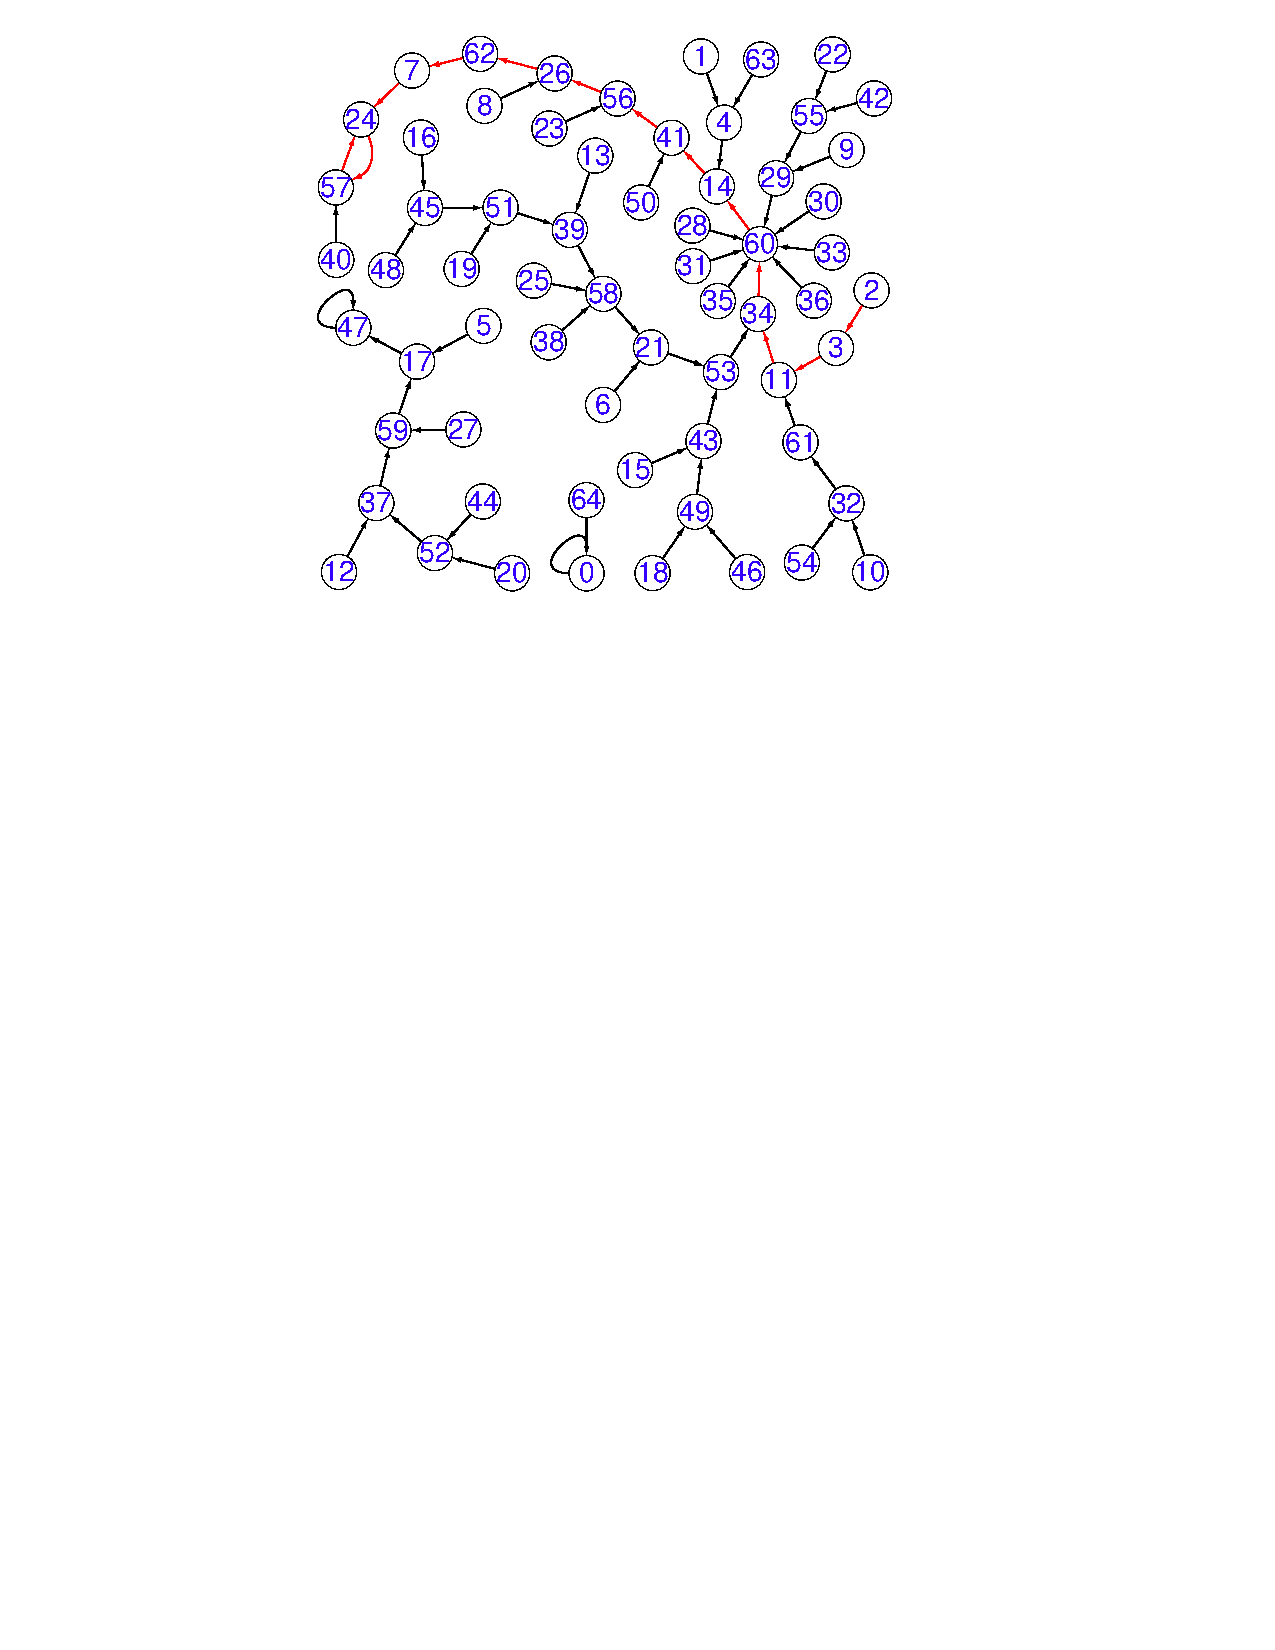
\includegraphics[width=\BigTwoImW]{state_perturbation}
a)
\end{minipage}\hspace{\figsep}
\begin{minipage}{0.97\BigTwoImW}
\centering
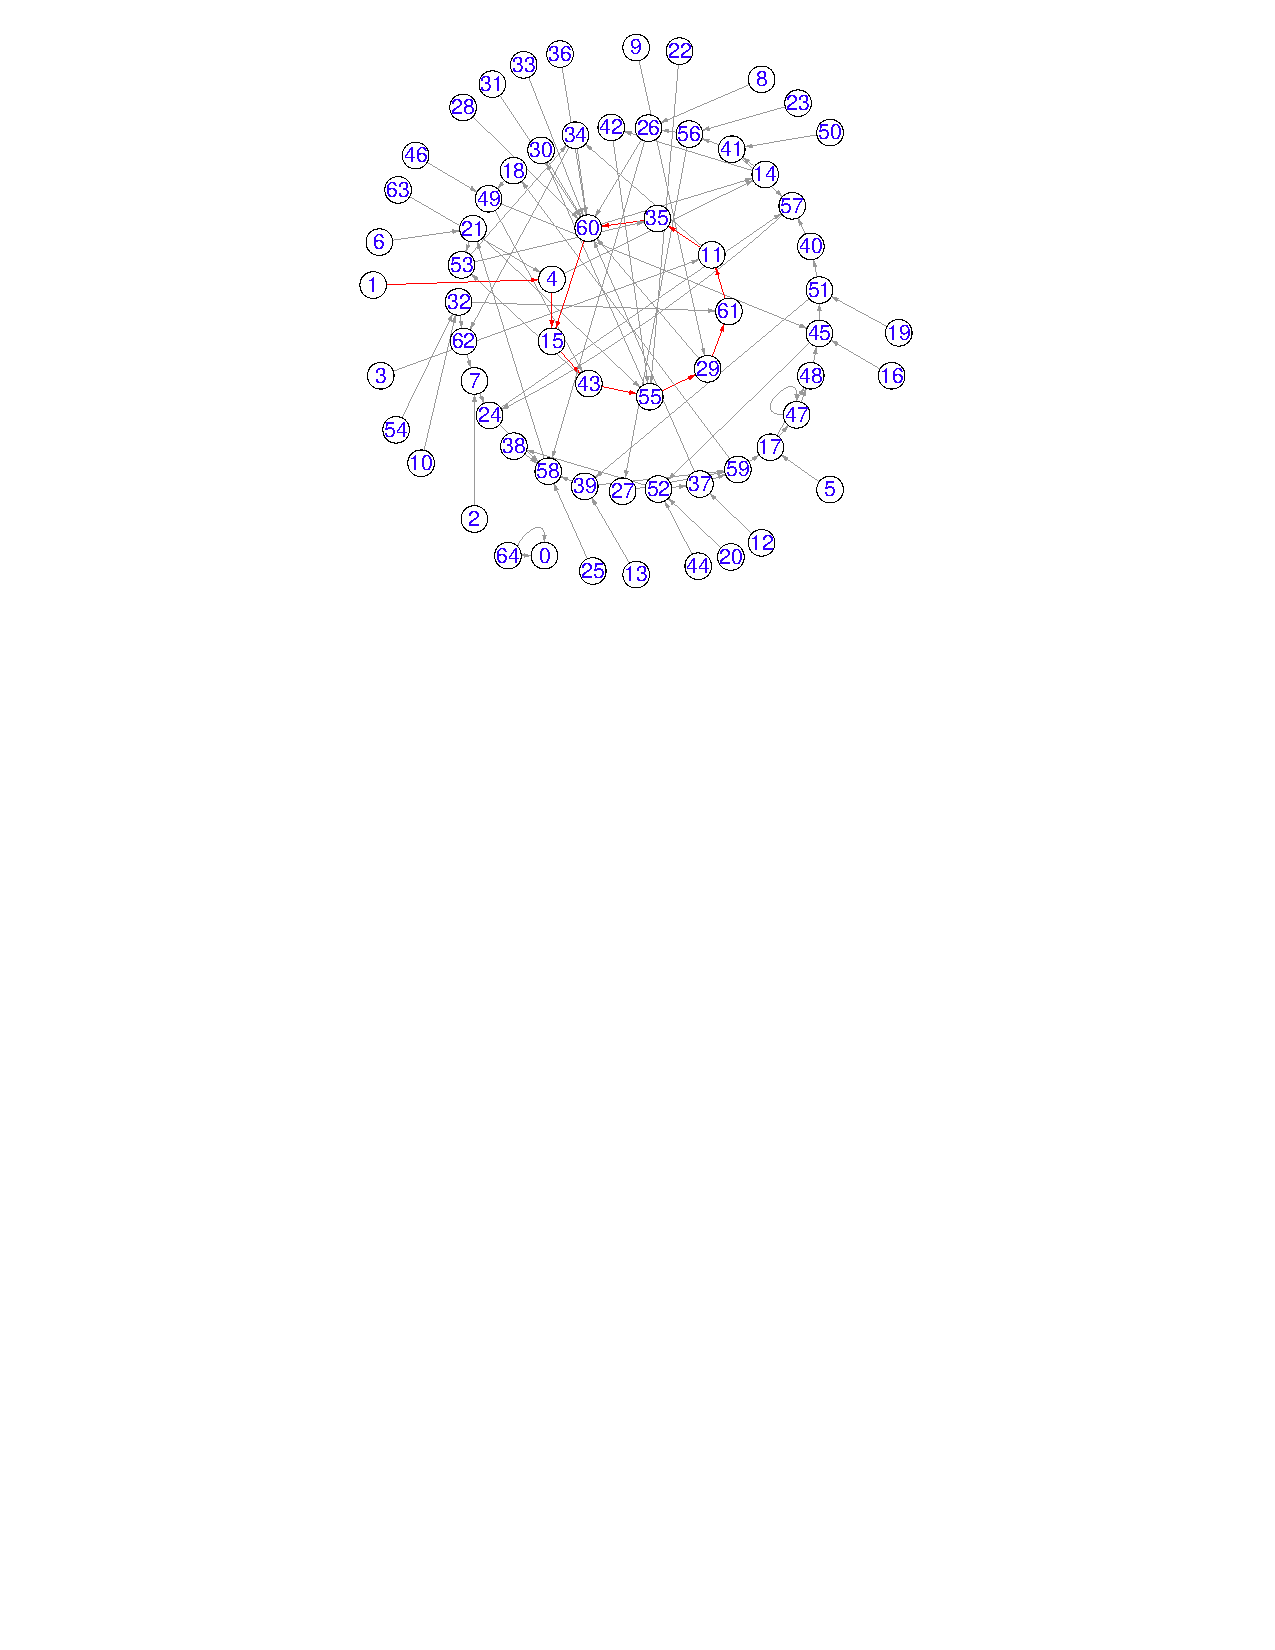
\includegraphics[width=0.97\BigTwoImW]{u_perturbation_sort}
b)
\end{minipage}\vspace{\figsep}
\begin{minipage}{\BigTwoImW}
\centering
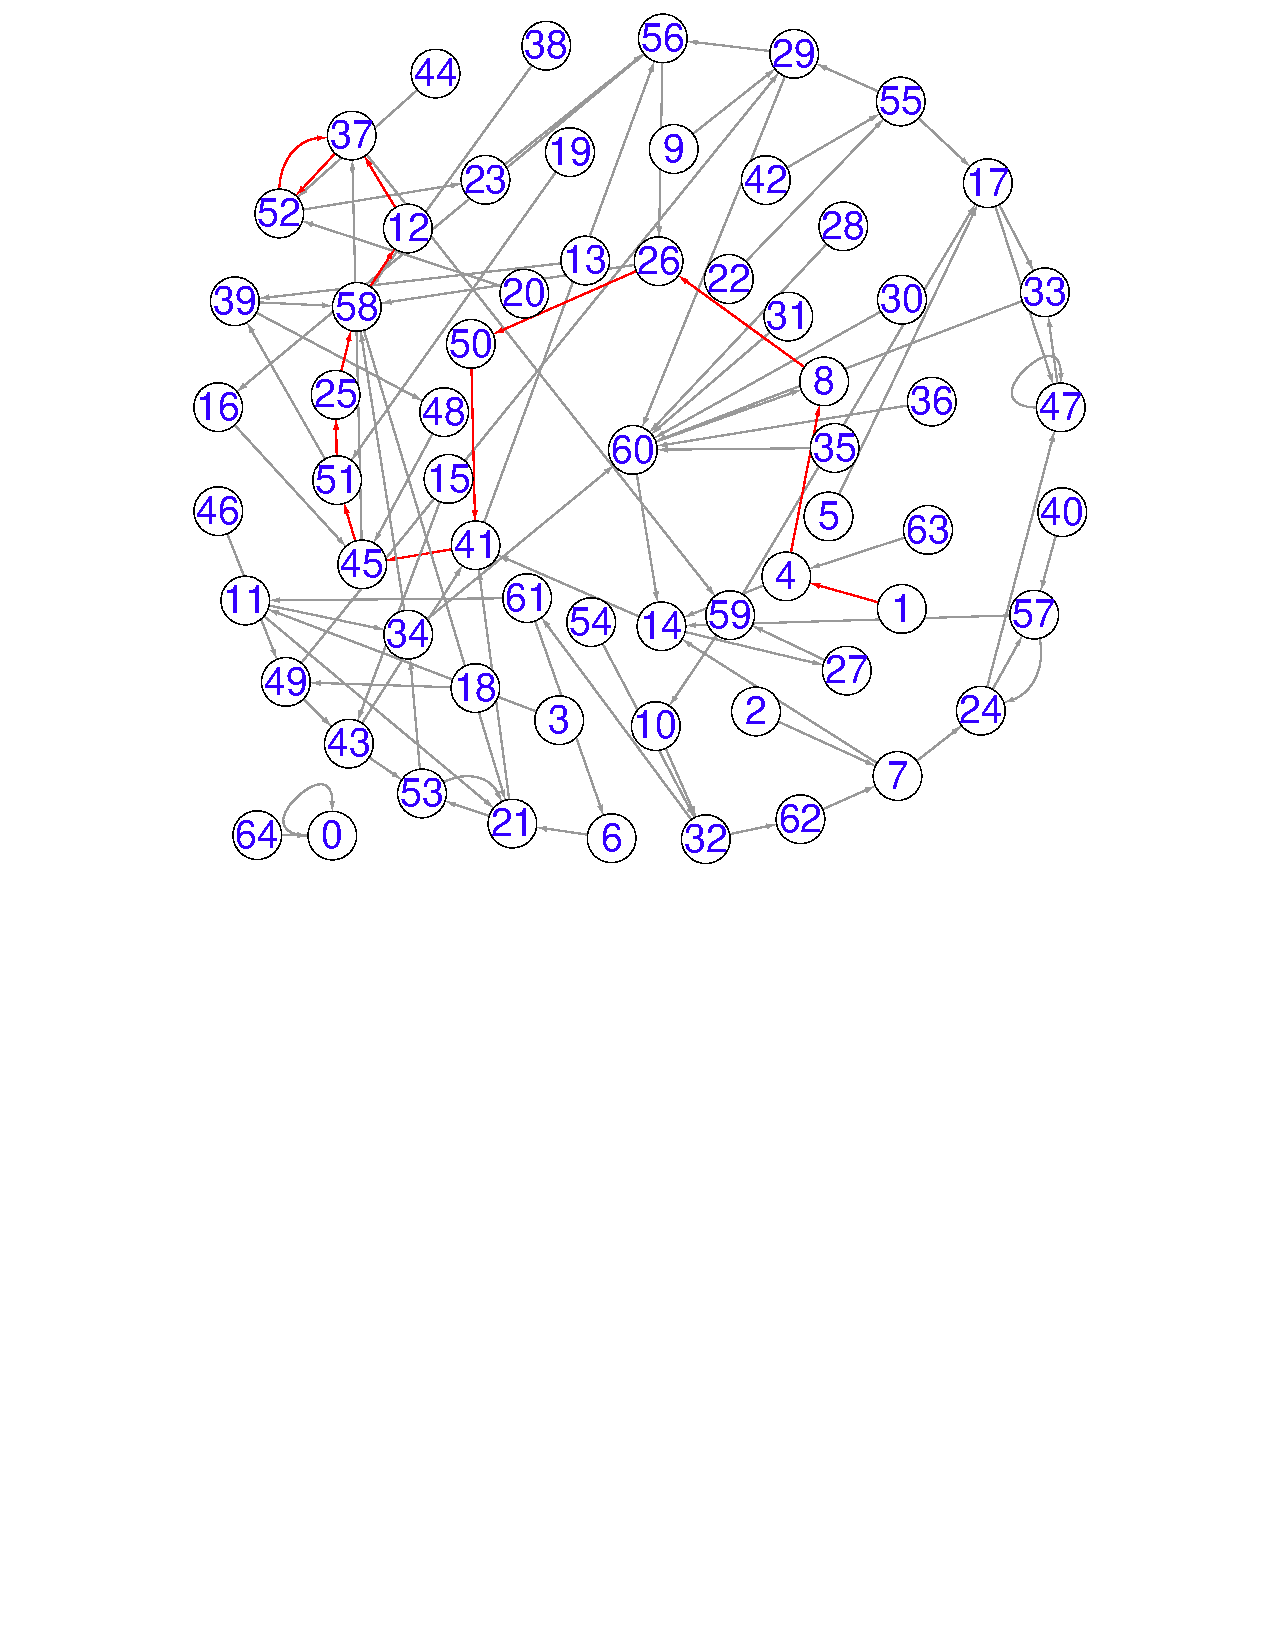
\includegraphics[width=\BigTwoImW]{DWSCS_sort}
c)
\end{minipage}\hspace{\figsep}
\begin{minipage}{0.965\BigTwoImW}
\centering
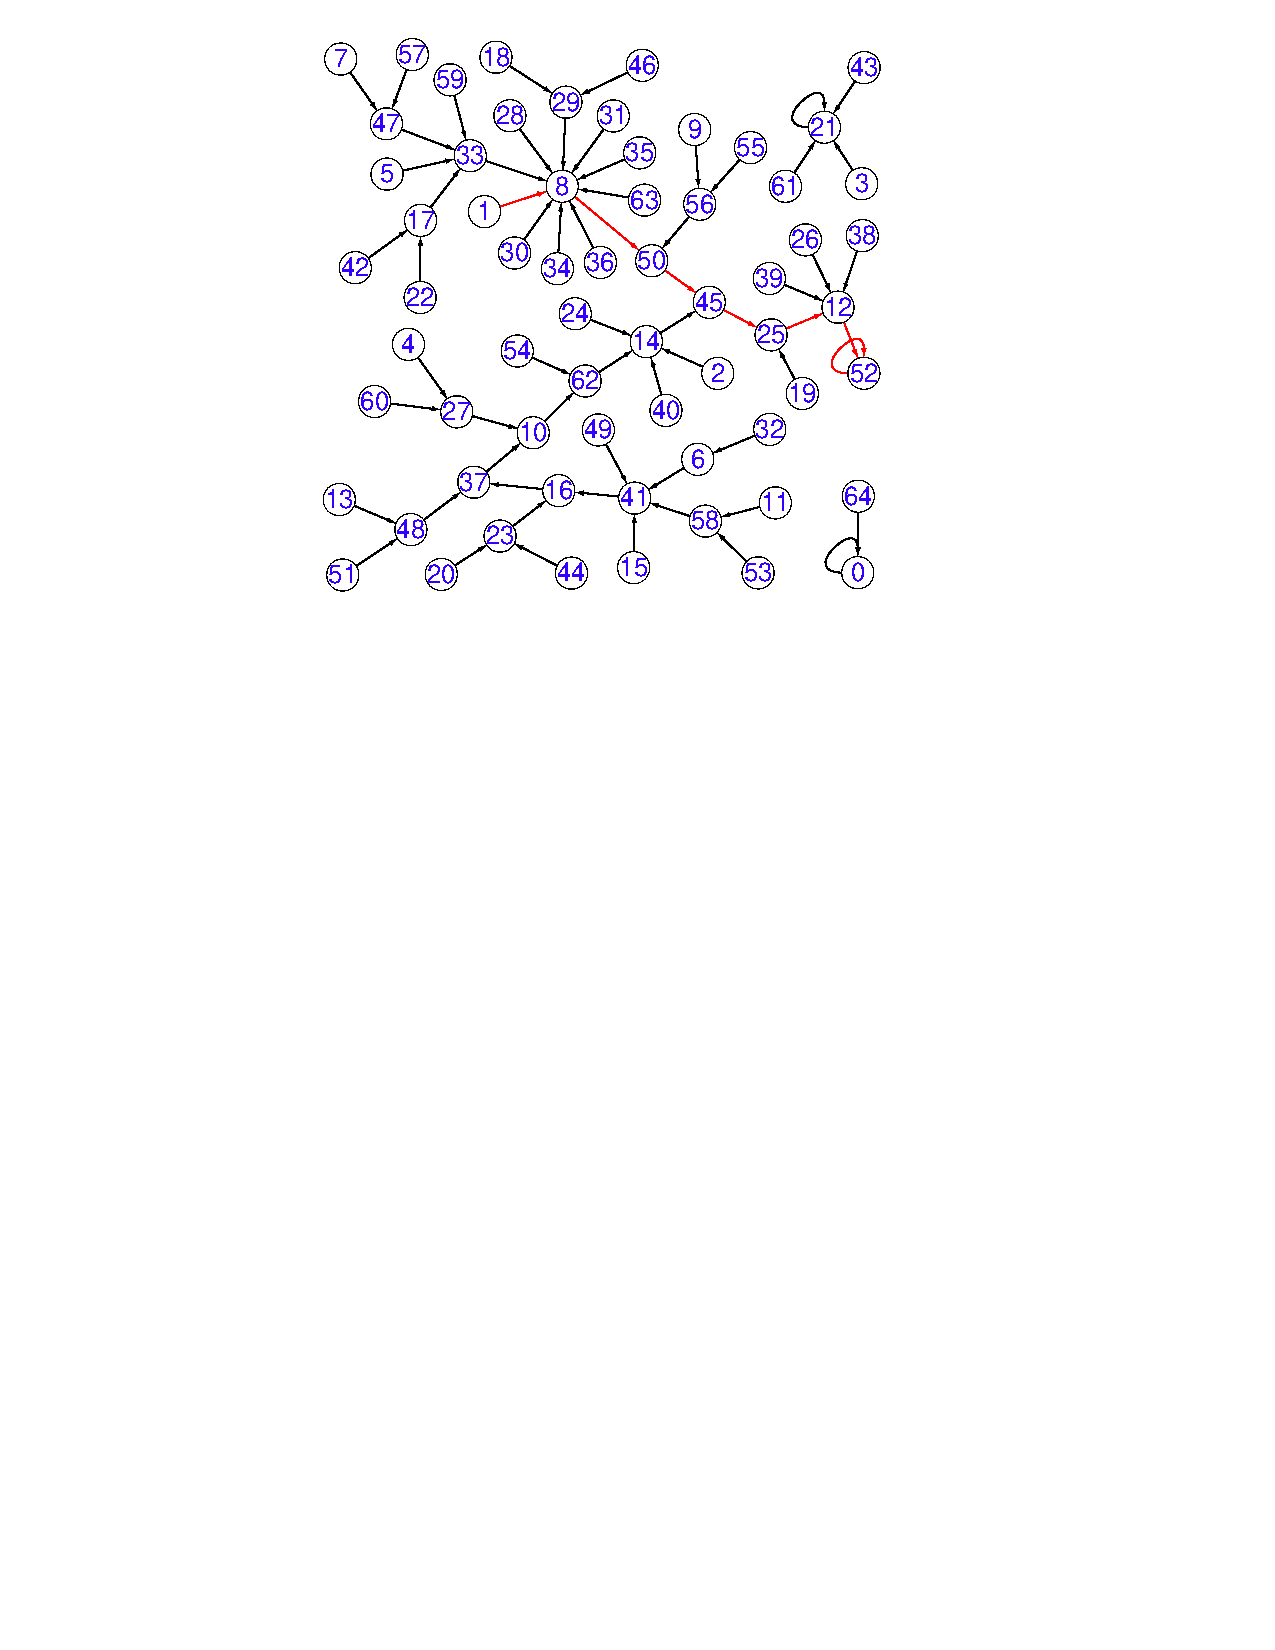
\includegraphics[width=0.965\BigTwoImW]{cascade_LT}
d)
\end{minipage}
\caption{对图~\ref{fig:networkLogistic5and6bits} b)对应SMN进行增强:
a) 扰动状态; b) 扰动控制参数; c) Logistic映射和Tent映射之间的转换; d) Logistic映射和Tent映射之间的级联}
\label{fig:networkMap6bits}
\end{figure*}

\item \textit{扰动控制参数}

扰动控制参数是指对控制参数不同的混沌系统状态映射网络进行级联\cite[Sec. 4]{vcernak1996digital}。以Logistic映射的状态映射网络
图~\ref{fig:networkLogistic5and6bits} b)、图~\ref{fig:networkLogistic8and6bits} b)为例,将上述两个状态映射网络
进行级联,扰动后状态映射网络如图~\ref{fig:networkMap6bits} b)所示。

\item \textit{混沌系统之间的转换}

混沌系统之间的转换是指在每次迭代中,交替改变混沌系统,前一个混沌系统的输出值为后一个混沌系统的输入值
\upcite{nagaraj2008increasing,YCZhou:Switching:TCASI2014}。
以本文分析讨论的Logistic映射和Tent映射为例,在其状态映射网络上交替跳转,转换后状态映射网络如图~\ref{fig:networkMap6bits} c)所示,
状态映射网络节点的最大入度与混沌系统的数量有关。

\item \textit{混沌系统之间的级联}

混沌系统之间的级联是指对不同混沌系统的状态映射网络进行级联\upcite{Hua:model:CAS17}。
1994年,Heidari等人提出了一种混沌系统级联方法,一个混沌系统的输出值为另一个混沌系统状态映射网络路径的起点\upcite{heidari1994chaotic}。
以Logistic映射和Tent映射为例,对图~\ref{fig:networkLogistic5and6bits} b)、图~\ref{fig:networkTent5and6bits} b)
对应的状态映射网络进行级联,级联后状态映射网络如图~\ref{fig:networkMap6bits} d)所示。根据图~\ref{fig:networkMap6bits} d)可以看出,
除孤立点$``0"$和$``2^n"$,整个状态映射网络单向连通。

\end{itemize}

\section{本章小结}

本章讨论了隐含在数字化Logistic映射中的一些动力学性质,首先利用整数量化函数准确推导出了Logistic映射的状态映射网络$F^*_{n}$与实现精度$n$之间的关系,
以累积入度为切入点理论上证明了定点运算域上Logistic映射的状态映射网络的无标度属性;其次,通过严格的数学推导,浮点运算域上系统量化误差对Logistic映射的影响被厘清,改变
Logistic映射中因式$x$与因式$(1-x)$的运算顺序可能使Logistic映射运算结果不同;最后,根据混沌映射的状态映射网络对基于混沌的伪随机数发生器发生器进行了分类,
研究发现,该分类方法可以粗检测混沌伪随机数发生器的随机性能。
